\begin{figure*}[t]
\centering
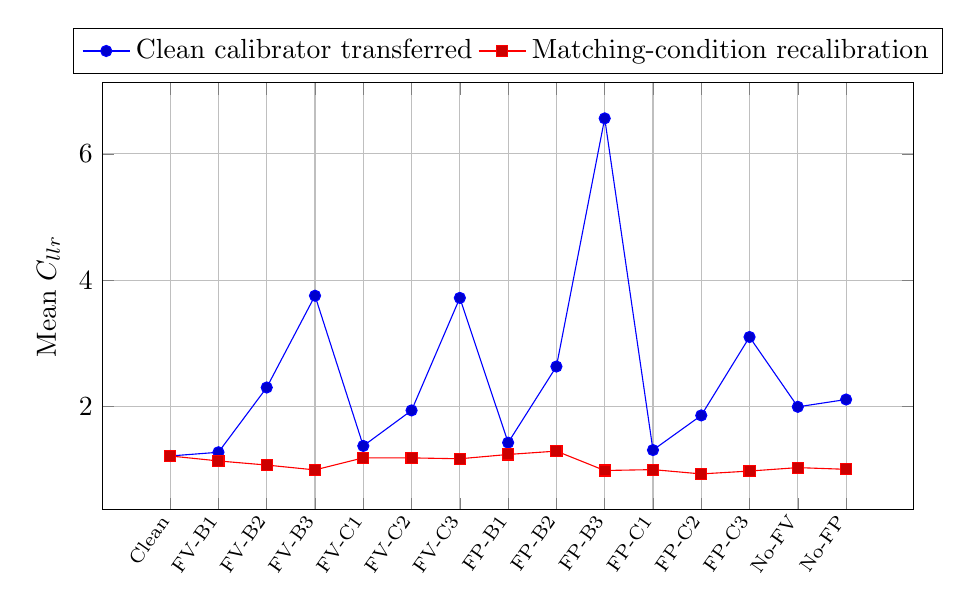
\begin{tikzpicture}
\begin{axis}[width=0.98\textwidth,height=7cm,ylabel={Mean $C_{llr}$},symbolic x coords={Clean,FV-B1,FV-B2,FV-B3,FV-C1,FV-C2,FV-C3,FP-B1,FP-B2,FP-B3,FP-C1,FP-C2,FP-C3,No-FV,No-FP},xtick=data,x tick label style={rotate=55,anchor=east,font=\scriptsize},grid=major,legend style={at={(0.5,1.02)},anchor=south,legend columns=2}]
\addplot coordinates {(Clean,1.215567) (FV-B1,1.274317) (FV-B2,2.299923) (FV-B3,3.753464) (FV-C1,1.374586) (FV-C2,1.937225) (FV-C3,3.719038) (FP-B1,1.426603) (FP-B2,2.632303) (FP-B3,6.562104) (FP-C1,1.309000) (FP-C2,1.857931) (FP-C3,3.099732) (No-FV,1.993928) (No-FP,2.109808)};
\addlegendentry{Clean calibrator transferred}
\addplot coordinates {(Clean,1.215567) (FV-B1,1.136864) (FV-B2,1.071614) (FV-B3,0.994705) (FV-C1,1.185755) (FV-C2,1.185091) (FV-C3,1.171241) (FP-B1,1.239374) (FP-B2,1.292585) (FP-B3,0.985440) (FP-C1,0.999372) (FP-C2,0.931326) (FP-C3,0.976730) (No-FV,1.031250) (No-FP,1.004154)};
\addlegendentry{Matching-condition recalibration}
\end{axis}
\end{tikzpicture}
\caption{Calibration robustness over the eight fusion systems. Matching-condition recalibration is diagnostic and does not replace the primary clean-calibrator transfer result.}
\label{fig:v1-calibration-transfer}
\end{figure*}
